\documentclass[dvipdfmx,11pt,a4paper]{jsbook}
\usepackage{package}
\usepackage{a4wide}
\usepackage[dvipdfmx]{hyperref}
\usepackage{pxjahyper}


%\title{}
%\author{}
%\date{\today}
\begin{document}
%\maketitle

%\tableofcontents

\makeatletter
\@addtoreset{equation}{section}
\def\theequation{\thesection.\arabic{equation}}
\makeatother


\chapter{CLASSICAL SOLITONS AND SOLITARY WAVES}
\begin{itembox}[l]{目的}
    非線形方程式の古典解のうち,ミンコフスキー計量やユークリッド方程式における場の方程式に対応するものがいくつかあり,そういった古典解から相対論的量子場の理論の情報を得る.
\end{itembox}

\section{Introduction}

本ゼミにおいてのメインテーマとなるソリトンとインスタントンであるが,どちらも簡単にいえば形状を保ったまま進行し互いに衝突・追突しても崩れないような局在化(localized)した波の事である.そもそもソリトンの英語スペルはsolitonであり,これはsolitary(孤立した)+on(粒子につける接尾辞(Fermi{\bf on}, Bos{\bf on}, Glu{\bf on}, Phot{\bf on} \dots))から来ている.すなわち孤立した波の塊でありながら歪むことなく安定に一様な速度で進行する波であり,粒子的に振る舞うような物理的対象を指す.ここで,なぜ局在化した波が粒子としてみなせるかということについては場の理論において場が作る波をエネルギーのたまり場のようなものであると捉えると,ポツンと局在化したエネルギーが非離散的(連続的)に形を崩さずに移動していればまるで粒子が移動していると拡大解釈できることから理解できる.

\begin{figure}[H]
    \centering
    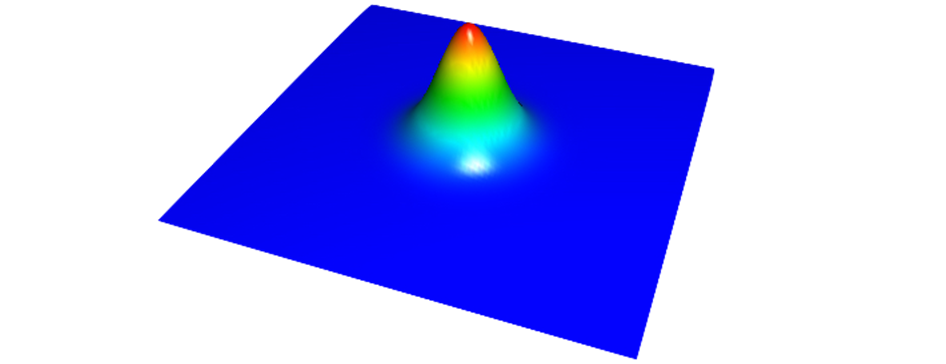
\includegraphics[width=8cm]{figure/soliton.png}
    \caption{ソリトン}
    \label{soliton}
\end{figure}


\end{document}
